\documentclass{../res/univ-projet}

%Import des packages utilisés pour le document
\usepackage[utf8x]{inputenc}
\usepackage[francais]{babel}
\usepackage[T1]{fontenc}
%\usepackage{array}
%\usepackage{hyperref}
%\usepackage{tabularx, longtable}
%\usepackage[table]{xcolor}
%\usepackage{fancyhdr}
%\usepackage{lastpage}
\usepackage{../res/tikz-uml}
\usepackage{tikz}
\usepackage{calc}
\usepackage{xstring}
\usepackage{pgfopts}

\definecolor{gris}{rgb}{0.95, 0.95, 0.95}

%Redéfinition des marges
%\addtolength{\hoffset}{-2cm}
%\addtolength{\textwidth}{4cm}
\addtolength{\topmargin}{-1cm}
\addtolength{\textheight}{1cm}
\addtolength{\headsep}{0.8cm} 
\addtolength{\footskip}{-0.2cm}


%Import page de garde et structures pour la gestion de projet
%\usepackage{structures}

%Variables
\logo{../res/logo_univ.png}
\title{Rapport de projet}
\author{\\ Pierre \bsc{Balmelle},\\ Lucas \bsc{Barbay}, \\ Matthieu \bsc{Fin},
\\ Olivier \bsc{Thibault}}
\projet{Projet PGP}
\projdesc{Étude et implantation d'un outil graphique de gestion de clefs PGP}
\filiere{Master 1 SSI }
\matiere{Conduite de projet}
\date{\today}

% -- Début du document -- %
\begin{document}

%Page de garde
\maketitle
\newpage
\thispagestyle{empty}
\setcounter{page}{0}
\section*{Remerciements}
Avant de débuter ce rapport, il nous parait indispensable de remercier les 
personnes qui ont contribué au bon déroulement de ce projet.

Nous remercions tout d'abord notre cliente, madame Magali BARDET, pour sa 
participation, son attention et la confiance qu'elle nous a accordée au 
cours de notre mission.

D'autre part, nos remerciements vont aussi à monsieur Karim ABDELLAH 
GODARD ainsi que monsieur Rémi DIONISI, pour la formation, le suivi 
et le soutien qu'ils nous ont apporté au cours de l'année.

Enfin, nous remercions l'ensemble de l'équipe enseignante du département 
informatique de Rouen, pour les connaissances qu'ils nous ont fournies lors 
de notre formation, sans quoi ce projet n'aurait pas eu lieu.
\newpage
\setcounter{page}{0}
%La table des matières
\tableofcontents

\newpage

\section{Introduction}

Au cours de notre première année de Master Informatique, un projet annuel 
en équipe nous a été confié afin de mettre en pratique ce qui nous a 
été enseigné dans l'unité ``Gestion de projet''. Il s'agit donc d'apprendre 
à s'organiser en équipe, faire preuve de méthodologie et d'adaptabilité 
pour mener à bien les objectifs d'un projet informatique. Ce rapport a pour 
but de présenter nos travaux durant ce projet.

Dans ce cadre, nous avons eu pour client Mme Magali BARDET, enseignante et 
responsable du Master Sécurité des Systèmes Informatiques (SSI) de l'UFR des 
Sciences et Techniques de Rouen. Notre mission s'est déroulée du 17 octobre 
2014 au 1\up{er} mai 2015. Durant cette période, nous avons été formés à la 
gestion de projet par M. Rémi DIONISI ainsi que M. Karim ABDELLAH GODARD.

Le thème de ce projet tourne autour d'OpenPGP. Le sujet se décompose en trois 
parties. La première partie consistait en la rédaction d'une étude d'OpenPGP 
et de son implantation en ligne de commande GnuPG. La deuxième partie a été 
l'implantation d'une interface graphique pour GnuPG. Enfin la troisième fut 
l'implantation et l'explication d'une attaque sur OpenPGP.

Dans un premier temps, il nous semble nécessaire de vous parler plus en 
détail du contexte de ce projet. Nous vous présenterons ensuite ce qui a été 
réalisé, puis nous ferons état des problèmes rencontrés. Enfin, pour finir 
nous effectuerons un bilan de ce projet.

\section{Contexte}
  \subsection{OpenPGP}
    OpenPGP est un standard normalisé dans la RFC 4880 qui définit des 
    formats de messages. Ces formats reposent sur de la cryptographie hybride, 
    c'est-à-dire une combinaison de clefs symétriques et asymétriques. Ils 
    permettent de fournir des services de sécurité pour les communications 
    électroniques ainsi que le stockage de données. Ces services quant à eux,
    oeuvrent pour garantir:
    \begin{itemize}
     \item la confidentialité (seuls les destinataires du message 
	   peuvent le déchiffrer),
     \item l'authenticité (l'émetteur d'un message est bien celui qu'il 
	   prétend être),
     \item l'intégrité (l'état des données transmises est le même qu'au 
	   moment de l'envoi, elles n'ont pas été altérées).
    \end{itemize}
 
  \subsection{GnuPG}
    GnuPG est une implémentation libre du standard OpenPGP. Ce logiciel a 
    pour but de proposer une alternative au logiciel PGP qui lui, est une
    implémentation non libre. 
    GnuPG permet de signer, vérifier (assure l'authenticité et l'intégrité), 
    chiffrer et déchiffrer (assure la confidentialité) des fichiers, ainsi 
    que de gérer un trousseau de clefs cryptographiques (asymétriques) 
    permettant ces actions. 
    Un modèle de toile de confiance est associé au trousseau de clefs. 
    Ce modèle permet de gérer pour chaque clef du trousseau une 
    validité pour garantir qu'elle appartient bien à la personne 
    identifiée, ainsi qu'un niveau de confiance en cette personne.
    
  \subsection{Le besoin}
    Il existe quelques interfaces graphiques (comme KGpg, GPA, Seahorse). 
    Cependant, ces interfaces ne permettent pas une gestion fine des clefs 
    et la partie toile de confiance n’est pas correctement représentée.
    Il nous a donc été demandé de proposer une interface graphique 
    permettant à un utilisateur novice en PGP, mais averti en sécurité, 
    de faire facilement des réglages techniques sur son trousseau et de pouvoir 
    mettre en place sa toile de confiance. Le logiciel doit donc être à la 
    fois pédagogique, précis et accompagné d'un document d’explications et 
    de recommandations d’utilisation. Il doit aussi fonctionner sous KDE et 
    gnome.
  
    Nous devions aussi réaliser une étude complète d'OpenPGP et du 
    logiciel GnuPG (en ligne de commande), d’en comprendre le 
    fonctionnement détaillé et de rédiger un rapport illustrant toutes 
    les fonctionnalités.

    Enfin, nous devions effectuer des recherches sur les limites 
    cryptographiques de PGP et produire un document d’analyse de ces 
    limites. En particulier il était demander d'implanter l’attaque sur les 
    identifiants de clefs PGP décrite dans le numéro 75 de MISC magazine.
    
  \subsection{Acteurs du projet}
    La cliente de ce projet est Mme Magali BARDET (enseignante et responsable 
    du master SSI à l'UFR des sciences et techniques de Rouen). 

    M. Karim Abdellah GODARD est un intervenant extérieur et a assuré le 
    rôle de formateur et consultant en gestion de projet.

    L'équipe en charge du développement était constituée de sept étudiants actuellement en première année du master IGIS de Rouen : 

    \begin{tabular}{ll}
    - Bertille BOUILLIE & Reponsable client \\
    - Guillaume LEROY & Architecte \\
    - Ibrahima Sory BARRY & Chargé client \\
    - Lucas BARBAY & Testeur \\
    - Matthieu FIN & Responsable technique \\
    - Pierre BALMELLE & Responsable qualité \\
    - Olivier THIBAULT & Chef de projet \\
    \end{tabular}
    
  \subsection{L'organisation}
    

\section{Présentation du projet}
    \subsection{Organisation}
    
    
    \begin{itemize}
      \item Ibrahima sur l'étude de GPG,
      \item Lucas sur l'attaque sur les KeyID,
      \item Les autres (Matthieu, Olivier et Pierre) sur le développement de l'application.
    \end{itemize}

  
  \subsection{L'interface graphique}
  
    Les fonctionnalités ayant été complétées sont :\medbreak
  \begin{itemize}
  
  \item Exécution d'actions GPG \smallbreak
  Création, exportation, importations de clés (en local)\smallbreak
  \item Chiffrer / déchiffrer / signer / vérifier \smallbreak
  Chiffrer ou déchiffrer ou signer ou vérifier un fichier. \smallbreak
  \item Affichage des commandes, des retours et des erreurs \smallbreak
  L'utilisateur peut choisir d'afficher ou non les commandes, les retours et les erreurs associés à chaque action GPG. \smallbreak 
  \item Création / Modification / Suppression du profil utilisateur \smallbreak
  \item Modification de la toile de confiance \smallbreak
  Modification de la toile de confiance par un changement de niveau de confiance, l'ajout d'une nouvelle clé ou la modification d'une clé.   
  \end{itemize}
 
   Les fonctionnalités qui ont été supprimées par rapport au plan initial sont :\medbreak
  \begin{itemize}
  \item Toile de confiance graphique\smallbreak
  Représentation de la toile de confiance sous forme de graphe\smallbreak
  \item Chiffrer / déchiffrer / signer / vérifier \smallbreak
  Chiffrer ou déchiffrer ou signer ou vérifier le texte contenu dans l'éditeur de l'interface.\smallbreak
  \item Edition de clé \smallbreak
  Quelques fonctions d'édition de clé ne sont pas implémentées, comme la révocation d'une clé ou la signature avec une clé en particulier \smallbreak 
  
  \end{itemize}

  La partie interface graphique a été validée par le client, l'attaque a été rendu mais non validée et l'étude n'a pas été rendu.
 
 \subsection{L'attaque}
  
  \subsubsection{Lexique}
  
  Avant de commencer l'attaque, il nous parait nécessaire d'expliquer quelques termes sur les clefs PGP :
  
  \begin{itemize}
  	\item Clef PGP : c'est une clef certification encapsulée dans un paquet PGP (défini dans la RFC 4880). La clef peut être une clef RSA ou une clef DSA.
	\item L'empreinte d'une clef : c'est l'image de la clef par la fonction de hachage sha-1 plus la date de création de cette clef et sa version. C'est d'ailleurs avec le champ de création que nous ferons l'attaque.
	\item L'identifiant d'une clef : c'est la troncature des 8 derniers caractères de l'empreinte.
  \end{itemize}
  
  
  Lors de l'importation d'une clef GPG par le biais d'un serveur, il est important de vérifier l'empreinte complète, c'est-à-dire les 40 caractères. Certaines personnes ne le font pas et se contentent de regarder seulement l'identifiant de la clef. L'attaque se base donc, non pas sur une faille de PGP, mais sur ce mauvais usage des utilisateurs non avertis. 
  
  L'objectif de l'attaque est donc de forger une clef pour tromper un utilisateur qui chercherait une clef sur le serveur et qui ne vérifierait pas la totalité de l'empreinte.
  
  \subsubsection{Le fonctionnement}

  L'attaque est issue du dépôt github trollwot fait par Micah Lee, lui-même faisant partie du projet Monkeysphere. Ce projet a pour but d'utiliser le standard OpenPGP pour d'autres utilisations comme l'identification avec SSH et HTTPS.
  
  Cette attaque est faite en Perl et reçoit plusieurs paramètres en entrée :
  
  \begin{itemize}
  	\item L'utilisateur, constitué d'un nom, prénom, adresse mail et d'un commentaire éventuellement. 
	\item L'identifiant de 8 caractères.
	\item La taille de la clef RSA (le script ne marche pas avec DSA).
  \end{itemize}

  Le principe de l'attaque est de changer la date de création jusqu'à avoir un identifiant identique.
  
  Le script commence par générer une clef RSA avec une date de création précise. Il récupère l'empreinte en appliquant la fonction de hachage sha-1 et l'identifiant en tronquant l'empreinte. Ensuite, on compare l'identifiant avec celui passé en paramètre. Si les deux sont différents, on fait varier la date de création et on recommence l'opération. On est obligé de décrémenter la date de création pour qu'elle soit conforme.
  
  Ce script est fait de façon mono thread et peut calculer environ 12 000 hachés par seconde sur les machines de l'université. Ce qui prend au maximum 4 jours pour couvrir les 2 \up{32} calculs nécessaires. 
  
  Lorsque le script trouve enfin un identifiant identique, il lui reste à construire un paquet PGP. Il utilise donc la clef RSA puis la dernière date de création pour former ce paquet.
    
  Pour tester ce script, nous avons tout d'abord généré une clef bobbb avec gpg.	  
  
  Nous avons lancé le script avec les mêmes informations que la clef générée.
  
  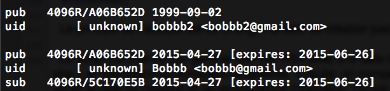
\includegraphics[scale=0.8]{clefs}
  
  Nous pouvons observer que les deux clefs ont le même identifiant.
  
  \subsubsection{Les contraintes de l'attaque}
  
      \begin{itemize}
        \item La date de création doit être supérieure à 1970 l'année 0 pour les machines.
        \item La date de création doit être inférieure à la date d'aujourd'hui.
      \end{itemize}
    \medbreak
    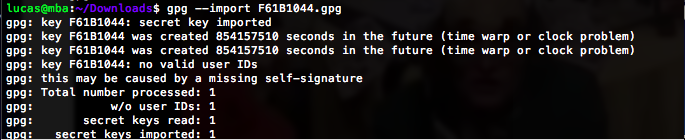
\includegraphics[scale=0.70]{attaque.png}

 On peut constater sur l'imprime écran ci-dessus qu'il existe une sécurité dans gpg qui vérifie la date des clefs. Nous avons eu une clef qui a été créée avec une date dans le futur et gpg refuse de l'importer dans notre trousseau.

\section{Les problèmes rencontrés}

  Lors de la réalisation de ce projet, nous avons dû faire face à
  différents problèmes aussi bien d'ordre organisationnel que techniques,
  auxquels nous avons dû remédier.

  \subsection{Problèmes organisationnels}

    Les difficultés organisationnelles rencontrées sont essentiellement
    survenues du fait de la modification de l'effectif de l'équipe durant la
    phase de réalisation du projet. 

    L'équipe initialement formée de sept développeurs
    s'est trouvée réduite de deux personnes :
    \begin{itemize}
      \item Bertille Bouillie qui dès les deux premières semaines n'a plus donné
      aucune nouvelle, son abandon a seulement pu être officiellement pris en compte au bout d'un mois et demi.
      \item Guillaume Leroy qui a abandonné le projet au bout d'un mois et demi.
    \end{itemize}

    De plus Guillaume avant son départ définitif a changé de formation avec Lucas pour intégrer le Master GIL
    ce qui nous a posé des difficultés d'emploi du temps pour réaliser les différentes réunions quotidiennes
    de l'équipe pour faire avancer le projet.

    De plus les actions entreprises lors de l'avant-projet n'ont pas suffi à l'ensemble de l'équipe 
    pour se former sur les différents outils utilisés lors de la phase de réalisation,
    puisque lors du premier sprint toutes les tâches attribuées à certains membres n'ont pas pu être
    réalisées suite à ces différentes lacunes.

    Nous avons, suite à cela pris du retard sur le premier sprint.

    Un plan d'action a alors été mis en place pour faire l'état des lieux des tâches
    faites, et des tâches réalisables avec le restant de l'équipe et le temps disponible.

    Ce plan a été présenté et discuté avec le client pour redéfinir le périmètre du projet.

    Suite à cela nous avons dû réattribuer les tâches à chacun pour pouvoir tenir la charge de travail,
    Lucas et Ibrahima ont souhaité se charger respectivement de l'attaque et de l'étude d'OpenPGP / GPG.

    Ainsi nous avons redéfini les tâches de développement de l'application
    entre Olivier, Matthieu (développeurs) et Pierre (Testeur).
    Les fonctionnalités de l'application ont également été redéfinies pour pouvoir être réalisables avec un effectif
    aussi réduit.

    De plus toute la réalisation de la visualisation de la toile de confiance a été réduite
    à l'affichage des niveaux de confiance d'une clé et non plus en dessin d'une toile de confiance graphique.

    Nous avons également à la fin du premier sprint suite à ces observations redéfini les rôles de chaque membre : 

    \begin{tabular}{|l|l|}
      \hline
      \bfseries{Noms}      & \bfseries{Rôles}                             \\
      \hline
      Olivier Thibault     & Chef de projet / Développeur                 \\
      Matthieu Fin         & Architecte / Chargé client / Développeur     \\
      Pierre Balmelle      & Testeur                                      \\
      Lucas Barbay         & Chargé de l'attaque                          \\
      Ibrahima Sorry Barry & Responsable de documentation OpenPGP / GnuPG \\
      \hline

    \end{tabular}

    
  \subsection{Problèmes techniques}

    \subsubsection{Maîtrise des outils}

      Lors de la phase d'avant projet nous avons organisé des sessions d’entraînement afin
      de prévenir du risque lié a l’incompréhension des outils utilisés tels que git, Qt, le langage C++,
      ou même le logiciel GnuPG.

      Seulement même si lors de l'avant-projet l'ensemble de l'équipe semblait maîtriser ces
      différents outils nous nous sommes rendu compte lors de la phase de développement que ce n'était pas le cas
      pour tout le monde.

      Les outils utilisés ont été définis conjointement dès le 27 novembre, or dès le début de la phase de développement
      (c'est à dire au mois de janvier) certains membres n'avaient toujours pas installé lesdits outils. Par conséquent
      ils ne pouvaient les maîtriser. Nous avons donc dû nous réunir pour installer et former a minima les différents membres
      sur ces outils, ce qui nous a fait perdre du temps sur le premier sprint de développement.

    \subsubsection{Maîtrise de GnuPG}
    
      Lors de la phase d'avant projet, nous avions seulement étudié le logiciel gpg
      en superficie, ce qui nous a valu quelques surprises lors du développement.

      Notamment tout le mécanisme de gestion des entrées / sorties du logiciel n'as pas vraiment été
      étudié, or la base de l'application demandée repose sur la gestion de la communication avec
      gpg.
      En effet celui-ci n'écrit et ne lit pas toujours sur son entrée et sa sortie standard,
      en fonction des paramètres qu'on lui donne.

      Et quand il ne lit ou n'écrit pas sur ses entrées / sortie standard il lit et écrit sur un
      tty.

      Nous avons donc dû trouver une solution à ce problème technique survenu lors du premier sprint,
      qui a consisté à développer une base de pseudo-terminal a l'aide de l'API POSIX, nous permettant
      d'exécuter un shell qui exécute gpg.
      Ainsi le shell s'occupe des descripteurs de fichier standard pour gpg et ce dernier peut accéder à un tty
      pour les commandes qui en nécessitent un.
      De plus notre pseudo terminal est composé d'une partie maître et d'une partie esclave,
      c'est la partie esclave qui s'occupe d'exécuter le shell avec gpg et la partie maître affiche
      sur sa sortie standard tout ce qui est écrit sur le terminal esclave, 
      et écrit sur le terminal esclave tout ce qui est écrit sur son entrée standard.

      Cela nous permet de regrouper tout ce qui est écrit et lu sur un même flux et donc de pouvoir
      complètement simuler l'exécution de commande gpg dans un terminal.
  

\section{Bilan du projet}
  
  \subsection{Compétences acquises}

    \subsubsection{Technique}
    
      Ce projet nous a beaucoup appris sur la partie technique du développement d'une interface graphique, en particulier l'utilisation du cadriciel (framework) Qt sous sa version 5, et de l'environnement de développement associé Qt Creator.

      Nous avons également gagné des compétences en C++, qui a été utilisé pour développer notre interface graphique.

      Les tests ont été l'occasion d'acquérir des connaissances sur le module Qt Test, et sur la manière d'effectuer des tests en général.

      Le projet a été l'occasion de découvrir GnuPG et ses nombreuses fonctionnalités.

    \subsubsection{Organisationnel}

      Nous avons retenu de ce projet qu'il est essentiel de s'assurer que l'équipe est effectivement formée sur les outils qui vont être utilisés ainsi que de faire l'inventaire de ces outils.
      
      Il faut aussi suivre régulièrement la progression de chaque membre dans la réalisation des tâches qui lui sont attribuées, pour être certain de l'état de progression de celles-ci et pouvoir s'adapter si elles ne sont pas finies à temps (ou finies plus tôt que prévu).




  \subsection{Axes d'amélioration}
  
    Le projet pourrait être amélioré en développant les commandes gpg prévues dans la STB initiale, mais qui ont dû être supprimées par manque de personnel, notamment pour l'édition de clé. 
    
    La toile de confiance graphique peut aussi être affichée sous forme de graphe, et offrir la possibilité de modifier une clé en effectuant un clic droit sur l'un des sommets du graphe (représentant une clé). 
    
    La personnalisation de l'interface pourrait être développée, donnant par exemple l'opportunité de personnaliser les couleurs représentant la validité ou la confiance d'une clé, ou les informations affichées sur chaque clé. 
    
    Le script de l'attaque peut également être amélioré. La recherche d'une nouvelle clef se fait en modifiant une clé générée et en comparant le haché de la modification jusqu'à ce qu'il corresponde à la clé ciblée. Selon les capacités de la machine, le script calcule entre 10 000 et 30 000 hachés par seconde, il faut donc plusieurs heures pour parcourir les $2^{32}$ possibilités. Les possibilités d'améliorations du script seraient donc de paralléliser les calculs ou d'utiliser la carte graphique pour effectuer plus de calculs.

  \subsection{Rétrospective}
	Si le projet était à refaire, il y a plusieurs choses que l'on ferait différemment. Nous commencerions par expérimenter le logiciel GnuPG en ligne de commande d'un point de vue utilisateur pour comprendre l'étendue de ces fonctionnalités. Ensuite nous ferions le nécessaire pour nous assurer que tous les membres de l'équipe ont une connaissance et une maîtrise suffisante des outils pour mener le projet à son terme.
	Si nous pouvions refaire ce projet, nous ne choisirions pas le langage c++. Nous nous tournerons plutôt vers le langage python qui nous aurait éviter entres autres un temps de compilation assez long, et augmenter notre productivité.

\section{Conclusion}

	Pour conclure ce rapport, nous pouvons dire que ce projet nous a permis de découvrir l'utilité des méthodes de gestion de projet dans une grosse équipe de 7 personnes. 
	
	La répartition des tâches dans une telle équipe est donc très importante et toutes les personnes doivent communiquer leur avancement sur le projet. 
	
	Nous avons décidé de réaliser ce projet avec la méthode agile Scrum qui consistait à séparait le projet en différents sprints en fonction de l'importance des tâches aux yeux du client. Pour avoir un bon suivi du projet, il était important de faire des réunions quotidiennes entre membres du projet et des réunions hebdomadaires avec le client. Ces méthodes agiles représentent un solide acquis, car elles nous serviront tout au long de notre vie professionnelle.
	
	GnuPG est un outil important dans le domaine de la messagerie sécurisé et avoir une expérience dans le domaine de la cryptographie nous ouvrira des portes lors de nos recherches de stage l'année prochaine. 
	
	Ce projet nous a également permis d'acquérir de nombreuses connaissances techniques telles que l'utilisation poussée du logiciel GPG, le développement en C++ et l'utilisation du cadriciel Qt, mais aussi des connaissances dans les outils collaboratifs tels que git ou encore slack (plateforme pour communiquer entre membres du projet).



\end{document}

